\chapter{โรคพืชที่เกิดจากจุลินทรีย์ กลไกระดับโมเลกุล และระบาดวิทยา}
\label{ch:plant_pathogens}

\begin{keyconcept}[แนวคิดสำคัญของบทที่ 4]
โรคพืชที่เกิดจากจุลินทรีย์สร้างความเสียหายทางเศรษฐกิจแก่ผลผลิตการเกษตรทั่วโลกมากกว่าร้อยละ 20--40 ต่อปี การเกิดโรคเป็นผลลัพธ์ของปฏิสัมพันธ์ 3 มิติใน "สามเหลี่ยมการเกิดโรคพืช" (Disease Triangle) ระหว่างพืชเจ้าบ้านที่อ่อนแอ จุลินทรีย์ก่อโรคที่มีความรุนแรง และสภาวะแวดล้อมที่เอื้ออำนวย ในระดับโมเลกุล การต่อสู้ระหว่างพืชและเชื้อก่อโรคดำเนินไปตามแบบจำลองทางภูมิคุ้มกันวิทยา "Zigzag Model" ซึ่งขับเคี่ยวระหว่างภูมิคุ้มกันกระตุ้นด้วยสารโมเลกุลก่อโรค (PTI) และการหลั่งโปรตีนแทรกซึม (Effectors) ผ่านระบบหลั่งสาร เช่น Type III Secretion System (T3SS) จนนำไปสู่ภูมิคุ้มกันตอบสนองจำเพาะ (ETI) การผสานแบบจำลองคณิตศาสตร์ระบาดวิทยา (AUDPC และ Logistic Model) ร่วมกับเทคโนโลยี Edge AI วิทัศน์คอมพิวเตอร์ ช่วยให้ตรวจจับและควบคุมการระบาดของโรคได้อย่างแม่นยำตั้งแต่ระยะเริ่มแรก
\end{keyconcept}

\begin{figure}[ht]
    \centering
    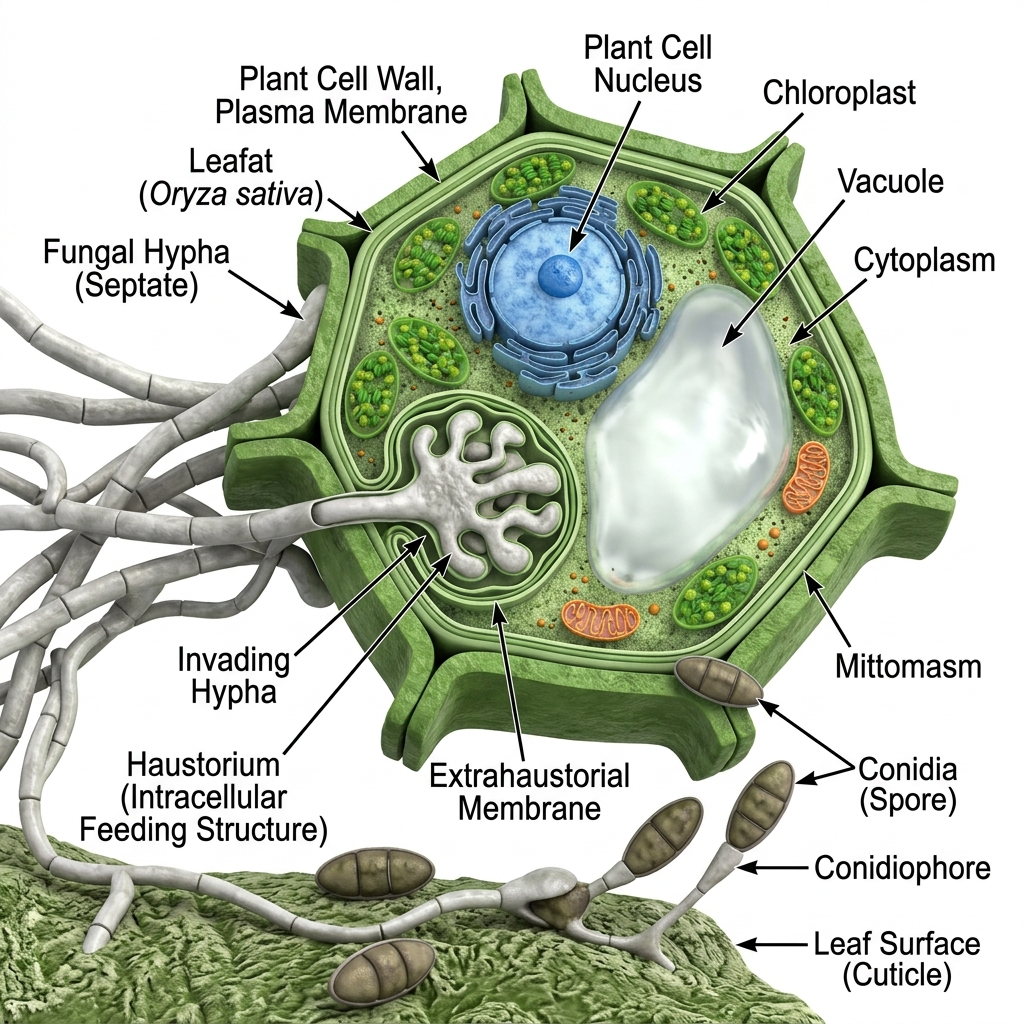
\includegraphics[width=0.85\textwidth]{assets/ch04_fungal_infection.png}
    \caption{การจำลองภาพ 3D ขยายส่วนปลายใยรา (Hypha) ขณะพัฒนาโครงสร้างแอพเพรสโซเรียม (Appressorium) สร้างแรงดันเต่งมหาศาล ส่งเข็มเจาะ (Penetration peg) ทะลุผนังเซลล์พืช และแผ่ขยายสายใยดูดซึมอาหารโฮสทอเรียม (Haustorium) โอบล้อมด้วยเยื่อหุ้มเซลล์โฮสต์โดยไม่ทำให้เยื่อหุ้มเซลล์แตกสลาย}
    \label{fig:ch04_fungal_infection}
\end{figure}

\section*{วัตถุประสงค์การเรียนรู้ประจำบท}
เมื่อศึกษาบทเรียนนี้จบแล้ว นักศึกษาสามารถ:
\begin{enumerate}
    \item อธิบายองค์ประกอบของสามเหลี่ยมการเกิดโรคพืช และพีระมิดโรคพืชที่บูรณาการมิติกาลเวลาและมนุษย์
    \item วิเคราะห์กลไกภูมิคุ้มกันพืชตามแบบจำลอง Zigzag Model (PTI vs ETS vs ETI) และระบบหลั่งสารของแบคทีเรียก่อโรค (T3SS, T4SS, T6SS)
    \item จำแนกสรีรวิทยาและกลไกการเข้าทำลายของเชื้อราแท้ ออยคาร์พิก (Oomycetes: \organism{Phytophthora}) แบคทีเรียท่อน้ำ และไวรัสพืช
    \item คำนวณแบบจำลองคณิตศาสตร์ระบาดวิทยา Monomolecular, Logistic และพื้นที่ใต้กราฟความรุนแรงของโรค (AUDPC)
    \item ประยุกต์ใช้เทคโนโลยี Edge AI และอัลกอริทึมวิทัศน์คอมพิวเตอร์ในการคัดกรองและประเมินระดับความรุนแรงของโรคพืชในแปลงเกษตรจริง
\end{enumerate}

\section{นิเวศวิทยาการเกิดโรค: สามเหลี่ยมและพีระมิดการเกิดโรคพืช}

การเกิดโรคในพืชไม่ได้ขึ้นอยู่กับเพียงแค่การมีอยู่ของเชื้อจุลินทรีย์เท่านั้น แต่เป็นปรากฏการณ์ทางนิเวศวิทยาที่ต้องอาศัยความสอดคล้องพร้อมกันของปัจจัยพื้นฐาน 3 ประการ ซึ่งรู้จักกันในนาม \textbf{สามเหลี่ยมการเกิดโรคพืช (Disease Triangle)\index{สามเหลี่ยมการเกิดโรคพืช (Disease Triangle)}}:

\begin{enumerate}
    \item \textbf{พืชเจ้าบ้านที่อ่อนแอ (Susceptible Host):} ระดับความอ่อนแอแปรผันตามพันธุกรรม อายุของพืช สภาพความสมบูรณ์ และระยะการเจริญเติบโต (เช่น ยอดอ่อนและผลอ่อนมักอ่อนแอกว่าใบแก่)
    \item \textbf{เชื้อก่อโรคที่มีความรุนแรงสูง (Virulent Pathogen):} ปริมาณหัวเชื้อเริ่มต้น (Inoculum density) ความสามารถในการสร้างสารพิษ เอนไซม์ย่อยผนังเซลล์ และความเร็วในการแบ่งตัวขยายพันธุ์
    \item \textbf{สภาพแวดล้อมที่เอื้ออำนวย (Favorable Environment):} อุณหภูมิ ความชื้นสัมพัทธ์ในอากาศ (RH $> 85\%$) ปริมาณน้ำฝน ความชื้นในดิน ค่า pH และการได้รับแสงแดด
\end{enumerate}

ในทางการเกษตรยุคใหม่ แบบจำลองสามเหลี่ยมได้รับการขยายเป็น \textbf{พีระมิดการเกิดโรคพืช (Disease Pyramid)\index{พีระมิดการเกิดโรคพืช (Disease Pyramid)}} โดยเพิ่มอีก 2 มิติสำคัญ:
\begin{itemize}
    \item \textbf{มิติของเวลา (Time):} ระยะเวลาที่พืชและเชื้อสัมผัสกันภายใต้สภาพแวดล้อมที่เหมาะสม ความถี่ของการเกิดหยดน้ำบนใบ (Leaf wetness duration)
    \item \textbf{กิจกรรมและการจัดการของมนุษย์ (Human Activity):} การปลูกพืชเชิงเดี่ยว (Monoculture) สายพันธุ์เดียวกันทั้งแปลง การให้ปุ๋ยไนโตรเจนมากเกินไปจนเนื้อเยื่อพืชอวบน้ำและอ่อนแอ ระบบการให้น้ำแบบสปริงเกอร์ที่กระจายสปอร์เชื้อรา และการเคลื่อนย้ายต้นพันธุ์ข้ามเขตแดน
\end{itemize}

\section{ภูมิคุ้มกันระดับโมเลกุลของพืช: แบบจำลอง Zigzag Model}

พืชไม่มีระบบภูมิคุ้มกันแบบแอนติบอดี (Adaptive Immune System) เหมือนสัตว์มีกระดูกสันหลัง แต่มีระบบภูมิคุ้มกันภายในระดับเซลล์ (Innate Immunity) ที่ซับซ้อน ซึ่งนักชีววิทยาพืช Jonathan Jones และ Jeffery Dangl (2006) ได้สรุปไว้เป็นแบบจำลองที่มีชื่อเสียงเรียกว่า \textbf{Zigzag Model\index{Zigzag Model of Plant Immunity}}:

\begin{figure}[ht]
\centering
\resizebox{0.96\textwidth}{!}{
\begin{tikzpicture}
    % Axes
    \draw[->, thick] (0,0) -- (12,0) node[right] {\textbf{เวลา (Time)}};
    \draw[->, thick] (0,0) -- (0,6) node[above] {\textbf{ภูมิคุ้มกัน (Amplitude)}};
    
    % Defense Thresholds
    \draw[dashed, red, thick] (0,2.5) -- (11.5,2.5);
    \node[red, font=\footnotesize\bfseries, above] at (6, 2.5) {ขีดขั้นการต้านทานโรค (Resistance Threshold)};
    
    % Zigzag Curve
    % Phase 1: PTI
    \draw[line width=1.8pt, blue] (0,0.5) -- (2.5,3.8) node[midway, above left, blue] {\textbf{1. PTI}};
    % Phase 2: ETS
    \draw[line width=1.8pt, red!80!black] (2.5,3.8) -- (5.0,1.2) node[midway, above right, red!80!black] {\textbf{2. ETS}};
    % Phase 3: ETI
    \draw[line width=1.8pt, forestgreen] (5.0,1.2) -- (8.0,5.5) node[midway, above left, forestgreen] {\textbf{3. ETI (HR)}};
    % Phase 4: Pathogen Evolution
    \draw[line width=1.8pt, orange] (8.0,5.5) -- (10.5,2.0) node[midway, above right, orange] {\textbf{4. Effector Div.}};
    \draw[line width=1.8pt, purple] (10.5,2.0) -- (11.8,4.8);
    
    % Labels below
    \node[draw, fill=blue!10, rounded corners, text width=2.4cm, align=center] at (1.5,-1.2) {\footnotesize \textbf{ระยะที่ 1}\\พืชตรวจจับ PAMPs ด้วย PRRs};
    \node[draw, fill=red!10, rounded corners, text width=2.4cm, align=center] at (4.5,-1.2) {\footnotesize \textbf{ระยะที่ 2}\\เชื้อหลั่ง Effectors ยับยั้ง PTI};
    \node[draw, fill=green!10, rounded corners, text width=2.4cm, align=center] at (7.8,-1.2) {\footnotesize \textbf{ระยะที่ 3}\\NBS-LRR จำจับ Effectors เกิด HR};
    \node[draw, fill=orange!10, rounded corners, text width=2.4cm, align=center] at (10.8,-1.2) {\footnotesize \textbf{ระยะที่ 4}\\เชื้อวิวัฒน์หลบหลีก พืชสร้าง R ใหม่};
\end{tikzpicture}
}
\caption{แบบจำลอง Zigzag Model แสดงการชิงไหวชิงพริบทางวิวัฒนาการระหว่างระบบภูมิคุ้มกันของพืชกับสารก่อโรคของจุลินทรีย์ (ดัดแปลงจาก Jones \& Dangl, 2006)}
\label{fig:zigzag_model}
\end{figure}

กลไกภูมิคุ้มกันของพืชประกอบด้วย 2 ชั้นหลัก:
\begin{enumerate}
    \item \textbf{PAMP-Triggered Immunity (PTI):\index{PAMP-Triggered Immunity (PTI)}} ชั้นภูมิคุ้มกันพื้นฐานที่ผิวนอกเซลล์ โดยตัวรับสัญญาณบนผิวเซลล์พืช (Pattern Recognition Receptors: PRRs) เช่น FLS2 (ตรวจจับแฟลกเจลลิน flg22 ของแบคทีเรีย) หรือ CERK1 (ตรวจจับไคตินของเชื้อรา) เมื่อตรวจพบสารโมเลกุลอนุรักษ์ของจุลินทรีย์ (Pathogen-Associated Molecular Patterns: PAMPs) พืชจะปิดปากใบ หลั่งสารกลุ่ม Reactive Oxygen Species (ROS burst) สะสมแคลเซียมไอออน ($Ca^{2+}$ flux) และกระตุ้นการสังเคราะห์สารพฤกษเคมีต้านเชื้อ (Phytoalexins)
    \item \textbf{Effector-Triggered Susceptibility (ETS):\index{Effector-Triggered Susceptibility (ETS)}} จุลินทรีย์ก่อโรคที่มีวิวัฒนาการขั้นสูงจะหลั่งโปรตีนที่เรียกว่า \textbf{Effectors} ข้ามเข้าสู่ไซโตพลาสซึมของเซลล์พืช เพื่อยับยั้งการส่งสัญญาณของ PRRs หรือทำลายโปรตีนภูมิคุ้มกันของพืช ส่งผลให้ภูมิคุ้มกัน PTI ล้มเหลวและเกิดโรคได้
    \item \textbf{Effector-Triggered Immunity (ETI):\index{Effector-Triggered Immunity (ETI)}} พืชมีโปรตีนต้านทานโรคภายในเซลล์ (Resistance proteins: R-proteins) ซึ่งส่วนใหญ่เป็นโปรตีนกลุ่ม \textbf{NBS-LRR (Nucleotide-Binding Site Leucine-Rich Repeat)} เข้าจับกับโปรตีน Effector โดยตรง หรือตรวจจับการเปลี่ยนแปลงของโปรตีนโฮสต์ที่ถูกโจมตี (Guard Hypothesis) การกระตุ้น ETI จะให้สัญญาณที่รวดเร็วและรุนแรง นำไปสู่ \textbf{การตอบสนองไวเกิน (Hypersensitive Response: HR)\index{Hypersensitive Response (HR)}} ซึ่งเป็นการทำให้เซลล์พืชบริเวณรอบแผลฆ่าตัวตาย (Programmed Cell Death) อย่างรวดเร็ว เพื่อกักกันเชื้อโรคไม่ให้แพร่กระจายไปยังเนื้อเยื่อปกติ
\end{enumerate}

\section{ระบบหลั่งโปรตีนก่อโรคของแบคทีเรีย (Bacterial Secretion Systems)}

แบคทีเรียก่อโรคพืชแกรมลบได้วิวัฒนาการระบบท่อระดับนาโนเมตริกเพื่อส่งโปรตีนก่อโรคและสารพิษเข้าสู่สิ่งแวดล้อมหรือเข้าสู่เซลล์พืชโดยตรง ระบบที่สำคัญอย่างยิ่งในโรคพืชได้แก่:

\subsection{1. ระบบหลั่งสารแบบที่ 3 (Type III Secretion System —T3SS)}
T3SS\index{Type III Secretion System (T3SS)} หรือที่เรียกว่า \textbf{Hrp pilus (Hypersensitive response and pathogenicity)} มีโครงสร้างทางสถาปัตยกรรมคล้าย ``เข็มฉีดยาขนาดนาโนเมตร'' ยื่นทะลุเยื่อหุ้มเซลล์ของแบคทีเรีย ผนังเซลล์ และเจาะทะลุผนังเซลล์ของพืชเข้าไปยังไซโตพลาสซึมโดยตรง แบคทีเรียกลุ่ม \organism{Pseudomonas syringae}, \organism{Ralstonia solanacearum}, และ \organism{Xanthomonas oryzae} ใช้ท่อนี้ในการฉีดโปรตีน Effector หลายสิบชนิดเข้าควบคุมกระบวนการทางสรีรวิทยาของพืช

\subsection{2. ระบบหลั่งสารแบบที่ 4 (Type IV Secretion System —T4SS)}
เป็นระบบที่สามารถส่งได้ทั้งโปรตีนและสารพันธุกรรม (DNA-protein complex)\index{Type IV Secretion System (T4SS)} ตัวอย่างคลาสสิกคือ \organism{Agrobacterium tumefaciens}\index{Agrobacterium tumefaciens@\textit{Agrobacterium tumefaciens}} ซึ่งใช้ T4SS ในการฉีดชิ้นส่วน T-DNA จาก Ti-plasmid เข้าไปเชื่อมต่อกับโครโมโซมของเซลล์พืช สั่งให้เซลล์พืชแบ่งตัวผิดปกติกลายเป็นปมเนื้องอก (Crown gall) และสังเคราะห์สารอาหารกลุ่มโอพีน (Opines) เลี้ยงแบคทีเรีย

\subsection{3. ระบบหลั่งสารแบบที่ 6 (Type VI Secretion System —T6SS)}
โครงสร้างมีลักษณะคล้ายหัวหอกและสปริงแบบ contractile bacteriophage tail\index{Type VI Secretion System (T6SS)} แบคทีเรียใช้ T6SS ในการแทงและฉีดสารพิษเข้าไปในเซลล์แบคทีเรียคู่แข่งหรือเซลล์ยูคาริโอต เพื่อครอบครองพื้นที่และแย่งชิงสารอาหารในไรโซสเฟียร์

\section{โรคพืชที่เกิดจากเชื้อราแท้และสิ่งมีชีวิตคล้ายรา (Oomycetes)}

\subsection{1. เชื้อราแท้ (True Fungi)}
เชื้อราแท้มีผนังเซลล์เป็นไคติน (Chitin) และ $\beta$-glucans มีรูปแบบการดำรงชีวิตแบบกินซาก (Necrotrophs), อิงอาศัยกับเนื้อเยื่อที่มีชีวิต (Biotrophs) หรือระยะแรกอยู่อาศัยแบบกลมกลืนก่อนฆ่าเนื้อเยื่อโฮสต์ในระยะต่อมา (Hemibiotrophs)

โครงสร้าง \textbf{Appressorium} ของเชื้อรา \organism{Magnaporthe oryzae} (ก่อโรคไหม้ข้าว) และ \organism{Colletotrichum gloeosporioides} (ก่อโรคแอนแทรคโนส) สามารถสร้างแรงดันเต่งภายใน (Turgor Pressure) ได้สูงถึง **8 เมกะปาสกาล (MPa)** หรือเทียบเท่ากับความดัน 80 บรรยากาศ โดยการสะสมสารกลีเซอรอลเข้มข้นสูงภายในเซลล์ แรงดันเต่งมหาศาลนี้จะผลักเข็มเจาะ (Penetration peg) ทะลุชั้นคิวทิเคิลของใบพืชได้อย่างง่ายดาย

\subsection{2. เชื้อโอไมซีตส์ (Oomycetes) และกรณีศึกษาโรครากเน่าโคนเน่าทุเรียน}

แม้จะมีลักษณะเส้นใยภายนอกคล้ายเชื้อรา แต่ในทางอนุกรมวิธาน \textbf{โอไมซีตส์ (Oomycetes)\index{โอไมซีตส์ (Oomycetes)}} จัดอยู่ในไฟลัม Stramenopiles หรือกลุ่ม Heterokonta ซึ่งใกล้ชิดกับสาหร่ายสีน้ำตาลมากกว่าเชื้อราแท้ ความแตกต่างสำคัญคือ:
\begin{itemize}
    \item ผนังเซลล์ประกอบด้วย **เซลลูโลสและ $\beta$-1,3/$\beta$-1,6-glucan** (แทบไม่มีไคติน)
    \item เส้นใยไม่มีผนังกั้น (Coenocytic hyphae)
    \item สร้างสปอร์ว่ายน้ำได้ที่มีแฟลกเจลลา 2 เส้น (Biflagellate zoospores)\index{ซูโอสปอร์ (Zoospores)} ซึ่งมีพฤติกรรมเคลื่อนที่เข้าหาสารเคมีจากรากพืช (Chemotaxis)
\end{itemize}

\begin{pathogen}[กรณีศึกษาเชิงลึก: การระบาดของ Phytophthora palmivora ในสวนทุเรียน จ.จันทบุรี และงานวิจัย RBRU]
เชื้อ \organism{Phytophthora palmivora}\index{Phytophthora palmivora@\textit{Phytophthora palmivora}}\index{โรครากเน่าโคนเน่าทุเรียน} เป็นเชื้อโอไมซีตส์ที่ก่อความเสียหายรุนแรงที่สุดต่ออุตสาหกรรมทุเรียนในภาคตะวันออกของประเทศไทย จากการสำรวจเชิงระบาดวิทยาในแปลงวิจัยของ Jantamalee \& Thassana (2026) \cite{jantamalee_2026_biotech} ครอบคลุม 40 สวนทุเรียนใน จ.จันทบุรี และ จ.ตราด พบว่าปัจจัยเร่งหลักเกิดจากฝนตกชุกต่อเนื่อง (ความชื้นดิน $>85\%$ ดินมีค่า $\text{pH } 4.6 - 5.2$) ซึ่งกระตุ้นการสร้างและว่ายน้ำของซูโอสปอร์ (Zoospores) เข้าสู่ระบบรากอย่างรวดเร็ว โดยเชื้อเข้าทำลาย 3 ส่วนหลัก:
\begin{itemize}
    \item \textbf{โรครากเน่า (Root Rot):} ซูโอสปอร์ว่ายเข้าหาปลายรากฝอย เข้าทำลายเนื้อเยื่อเปลือกราก ทำให้รากฝอยเน่าเปื่อยเป็นสีน้ำตาลดำ พืชสูญเสียความสามารถในการดูดน้ำและธาตุอาหาร ส่งผลให้ยอดแห้งตายจากบนลงล่าง (Dieback)
    \item \textbf{โรคลำต้นเน่าและเปลือกเน่า (Stem Canker / Gummosis):} เชื้อเข้าทำลายเนื้อเยื่อท่อลำเลียงใต้เปลือกไม้ ทำให้เปลือกแตก ปรากฏรอยแผลช้ำสีน้ำตาลเข้ม และมีหยดน้ำยางสีน้ำตาลแดงเยิ้มไหลซึมออกมา
    \item \textbf{โรคผลเน่า (Fruit Rot):} เชื้อกระเซ็นจากผิวดินขึ้นสู่ผลทุเรียนในช่วงฝนตกชุก เกิดรอยแผลสีน้ำตาลไหม้ขอบแผลมีเส้นใยสีขาวฟู ลุกลามจนเนื้อทุเรียนเน่าเสียส่งกลิ่นเปรี้ยว
\end{itemize}
เพื่อการเฝ้าระวังเชิงรุก คณะผู้วิจัย มรภ.รำไพพรรณี ได้พัฒนาเทคนิคตรวจยีนจำเพาะ \textit{Ypt1} ด้วยวิธี Rapid PCR ร่วมกับระบบภาพวิทัศน์ Edge AI \cite{tsana2026edge}\index{งานวิจัย RBRU!โรครากเน่าโคนเน่าทุเรียน} ที่สามารถระบุการติดเชื้อได้ตั้งแต่ระยะแฝงตัว (Latent phase) ก่อนที่เนื้อเยื่อท่อลำเลียงจะถูกทำลายถาวร
\end{pathogen}

\section{โรคพืชที่เกิดจากแบคทีเรียและไวรัส}

\subsection{1. แบคทีเรียก่อโรคพืชสำคัญ}
\begin{itemize}
    \item \textbf{โรคเหี่ยวเขียว (Bacterial Wilt):\index{โรคเหี่ยวเขียว (Bacterial Wilt)}} เกิดจาก \organism{Ralstonia solanacearum}\index{Ralstonia solanacearum@\textit{Ralstonia solanacearum}} เข้าสู่พืชทางบาดแผลราก แล้วเข้าไปเพิ่มจำนวนมหาศาลในท่อน้ำ (Xylem) แบคทีเรียสร้างสารพอลิเมอร์เมือกนอกเซลล์ (Exopolysaccharides: EPS) อุดตันท่อลำเลียงน้ำ ทำให้พืชเหี่ยวเฉียบพลันขณะใบยังเขียว การตรวจสอบภาคสนามทำได้ง่ายโดยการตัดลำต้นแช่ในน้ำใส จะสังเกตเห็นสายเมือกแบคทีเรียสีขาวขุ่น (Bacterial stream / ooze) ไหลออกจากปลายท่อ
    \item \textbf{โรคขอบใบแห้งข้าว (Bacterial Blight):\index{โรคขอบใบแห้งข้าว}} เกิดจาก \organism{Xanthomonas oryzae} pv. \textit{oryzae}\index{Xanthomonas oryzae@\textit{Xanthomonas oryzae}} เข้าทำลายทางรูเปิดธรรมชาติ เช่น ไฮดาโทด (Hydathode) ทำให้ขอบใบข้าวแห้งเป็นทางยาวสีฟางข้าว
    \item \textbf{โรคแคงเกอร์ส้ม (Citrus Canker):\index{โรคแคงเกอร์ส้ม}} เกิดจาก \organism{Xanthomonas citri} subsp. \textit{citri} แผลตกสะเก็ดนูนสีน้ำตาล มีวงสีเหลือง (Yellow halo) ล้อมรอบบนใบ กิ่ง และผลส้ม
\end{itemize}

\subsection{2. ไวรัสพืชและพาหะแมลง}
ไวรัสพืชส่วนใหญ่มีสารพันธุกรรมเป็น single-stranded RNA (ssRNA) ไม่สามารถเจาะผ่านผนังเซลล์พืชได้ จึงต้องอาศัยแมลงปากดูดเป็นพาหะ:
\begin{itemize}
    \item \textbf{Tobacco Mosaic Virus (TMV):} ไวรัสรูปท่อน มีเสถียรภาพสูงมาก ทนความร้อนและสารเคมี ถ่ายทอดผ่านการสัมผัสและรอยขีดข่วนของใบ
    \item \textbf{Tomato Yellow Leaf Curl Virus (TYLCV):} ไวรัสในวงศ์ Geminiviridae ถ่ายทอดโดยแมลงหวี่ขาว (\organism{Bemisia tabaci}) ทำให้ใบมะเขือเทศหงิกงอ ยอดตั้งชัน ขอบใบเหลือง และหยุดการเจริญเติบโต
\end{itemize}
ไวรัสเคลื่อนที่ข้ามเซลล์พืชผ่านช่องเชื่อมไซโตพลาสซึม **พลาสโมเดสมาตา (Plasmodesmata)** โดยอาศัยโปรตีนเคลื่อนที่ (Movement Proteins: MP) ทำหน้าที่ขยายขนาดช่องพลาสโมเดสมาตาให้กรดนิวคลีอิกของไวรัสลอดผ่านได้

\section{ระบาดวิทยาเชิงปริมาณและแบบจำลองคณิตศาสตร์โรคพืช}

J.E. van der Plank (1963) บิดาแห่งระบาดวิทยาโรคพืชยุคใหม่ ได้จำแนกโรคพืชตามจลนศาสตร์ของการแพร่ระบาดออกเป็น 2 รูปแบบหลัก:

\subsection{1. แบบจำลองมอนอโมเลกุลาร์ (Monomolecular Model)}
ใช้สำหรับโรคพืชแบบ \textbf{วงจรเดียว (Monocyclic Disease)} ซึ่งเชื้อก่อโรคไม่มีการสร้างสปอร์ขยายพันธุ์ข้ามต้นซ้ำในฤดูปลูกเดียวกัน (Inoculum เกิดจากแหล่งเดิมในดิน เช่น โรคเหี่ยวจากเชื้อราในดิน):

\begin{equation}
\frac{dy}{dt} = r_m (1 - y)
\end{equation}

เมื่อ $y$ คือสัดส่วนของเนื้อเยื่อหรือต้นพืชที่เป็นโรค ($0 \le y \le 1$), $t$ คือเวลา (วัน), และ $r_m$ คืออัตราการติดเชื้อแบบมอนอโมเลกุลาร์ (ต่อวัน) เมื่อทำการอินทิเกรตจะได้:

\begin{equation}
\ln\left(\frac{1}{1 - y}\right) = \ln\left(\frac{1}{1 - y_0}\right) + r_m t
\end{equation}

\subsection{2. แบบจำลองโลจิสติก (Logistic Model)}
ใช้สำหรับโรคพืชแบบ \textbf{หลายวงจร (Polycyclic Disease)}\index{แบบจำลองโลจิสติก (Logistic Disease Model)} ซึ่งเชื้อสามารถสร้างสปอร์รุ่นใหม่แพร่กระจายและติดเชื้อซ้ำในแปลงได้หลายรอบในหนึ่งฤดูกาล (เช่น โรคไหม้ข้าว ราสนิม ราน้ำค้าง):

\begin{equation}
\frac{dy}{dt} = r_l \, y (1 - y)
\end{equation}

เมื่อ $r_l$ คืออัตราการติดเชื้อสัมพัทธ์ (Apparent infection rate) กราฟการระบาดจะเป็นรูปตัวเอส (Sigmoid curve) เมื่อทำการอินทิเกรตจะได้สมการแปลงค่าลอจิต (Logit transformation):

\begin{equation}
\text{logit}(y) = \ln\left(\frac{y}{1 - y}\right) = \ln\left(\frac{y_0}{1 - y_0}\right) + r_l t
\end{equation}

\subsection{3. พื้นที่ใต้กราฟความก้าวหน้าของโรค (AUDPC)}
การเปรียบเทียบประสิทธิภาพของการควบคุมโรค หรือการทดสอบพันธุ์พืชต้านทาน นิยมประเมินผ่าน \textbf{พื้นที่ใต้กราฟความก้าวหน้าของโรค (Area Under the Disease Progress Curve: AUDPC)\index{AUDPC (Area Under Disease Progress Curve)}}:

\begin{equation}
\text{AUDPC} = \sum_{i=1}^{n-1} \left[ \frac{y_i + y_{i+1}}{2} \right] (t_{i+1} - t_i)
\end{equation}

เมื่อ $y_i$ คือระดับความรุนแรงของโรค ณ เวลาการประเมินครั้งที่ $i$, $t_i$ คือเวลาการประเมิน (วัน) และ $n$ คือจำนวนครั้งทั้งหมดที่ทำการตรวจวัด

\begin{worked}[ตัวอย่างที่ 4.1 การวิเคราะห์อัตราการระบาดโลจิสติก (Logistic Model) ในโรคใบไหม้ทุเรียน]
ในการติดตามการระบาดของโรคใบไหม้ทุเรียนในแปลงทดลอง จ.จันทบุรี:
\begin{itemize}
    \item ณ วันที่ 0 ($t_0 = 0$) สัดส่วนใบที่เป็นโรคเริ่มต้น $y_0 = 0.02$ (2\%)
    \item หลังจากผ่านไป 20 วัน ($t = 20$) ในแปลงที่ไม่ได้พ่นชีวภัณฑ์ สัดส่วนใบเป็นโรคเพิ่มขึ้นเป็น $y = 0.35$ (35\%)
\end{itemize}
จงคำนวณหาอัตราการติดเชื้อปรากฏ ($r_l$) ของแปลงดังกล่าว และทำนายสัดส่วนใบเป็นโรค ณ วันที่ 35 หากไม่มีการควบคุมโรค

\textbf{วิธีทำ:}
1. คำนวณหาอัตราการติดเชื้อ $r_l$:
$$\ln\left(\frac{y_0}{1 - y_0}\right) = \ln\left(\frac{0.02}{0.98}\right) = \ln(0.0204) \approx -3.892$$
$$\ln\left(\frac{y}{1 - y}\right) = \ln\left(\frac{0.35}{0.65}\right) = \ln(0.5385) \approx -0.619$$
จากสมการ $\text{logit}(y) = \text{logit}(y_0) + r_l t$:
$$-0.619 = -3.892 + r_l (20)$$
$$20 \, r_l = 3.892 - 0.619 = 3.273 \implies r_l = \frac{3.273}{20} \approx 0.1636 \text{ ต่อวัน}$$

2. ทำนายความรุนแรงของโรค ณ วันที่ $t = 35$:
$$\text{logit}(y_{35}) = -3.892 + (0.1636 \times 35) = -3.892 + 5.726 = 1.834$$
$$\frac{y_{35}}{1 - y_{35}} = e^{1.834} \approx 6.259$$
$$y_{35} = \frac{6.259}{1 + 6.259} = \frac{6.259}{7.259} \approx 0.862 \text{ หรือ } 86.2\%$$

\textbf{บทวิเคราะห์ผลลัพธ์:} อัตราการติดเชื้อ $r_l = 0.164$ ต่อวัน บ่งชี้การระบาดระดับรุนแรงมาก หากเกษตรกรปล่อยทิ้งไว้โดยไม่พ่นควบคุมชีวภัณฑ์ เพียง 35 วัน ใบพืชในแปลงจะได้รับความเสียหายสูงถึง 86.2\% ส่งผลให้ต้นทุเรียนผลัดใบทั้งหมดและยืนต้นตาย
\end{worked}

\begin{worked}[ตัวอย่างที่ 4.2 การคำนวณ AUDPC เปรียบเทียบประสิทธิภาพการใช้ราปฏิปักษ์ \organism{Trichoderma}]
นักวิจัยประเมินความรุนแรงของโรคแผลสะเก็ดบนผลทุเรียน ($0 \le y \le 1$) ทุกๆ 7 วัน เป็นเวลา 21 วัน ระหว่างแปลงใช้สารเคมีสังเคราะห์กับแปลงพ่นชีวภัณฑ์สปอร์สด \organism{Trichoderma harzianum}:

\begin{center}
\small
\begin{tabular}{ccccc}
\toprule
\textbf{กรรมวิธี} & \textbf{วันที่ 0 ($t_1$)} & \textbf{วันที่ 7 ($t_2$)} & \textbf{วันที่ 14 ($t_3$)} & \textbf{วันที่ 21 ($t_4$)} \\
\midrule
ชุดควบคุม (ไม่อินอคูเลต) & 0.05 & 0.18 & 0.42 & 0.70 \\
พ่น \organism{Trichoderma} & 0.05 & 0.09 & 0.15 & 0.22 \\
\bottomrule
\end{tabular}
\end{center}

จงคำนวณค่า AUDPC ของทั้งสองกรรมวิธี และร้อยละการลดความเสียหายของโรค

\textbf{วิธีทำ:}
1. คำนวณ AUDPC ของชุดควบคุม:
$$\text{ช่วงที่ 1 } (0-7 \text{ วัน}): \left(\frac{0.05 + 0.18}{2}\right) \times 7 = 0.115 \times 7 = 0.805$$
$$\text{ช่วงที่ 2 } (7-14 \text{ วัน}): \left(\frac{0.18 + 0.42}{2}\right) \times 7 = 0.300 \times 7 = 2.100$$
$$\text{ช่วงที่ 3 } (14-21 \text{ วัน}): \left(\frac{0.42 + 0.70}{2}\right) \times 7 = 0.560 \times 7 = 3.920$$
$$\text{AUDPC}_{\text{Control}} = 0.805 + 2.100 + 3.920 = 6.825 \text{ day-fraction}$$

2. คำนวณ AUDPC ของแปลงพ่น \organism{Trichoderma}:
$$\text{ช่วงที่ 1 } (0-7 \text{ วัน}): \left(\frac{0.05 + 0.09}{2}\right) \times 7 = 0.070 \times 7 = 0.490$$
$$\text{ช่วงที่ 2 } (7-14 \text{ วัน}): \left(\frac{0.09 + 0.15}{2}\right) \times 7 = 0.120 \times 7 = 0.840$$
$$\text{ช่วงที่ 3 } (14-21 \text{ วัน}): \left(\frac{0.15 + 0.22}{2}\right) \times 7 = 0.185 \times 7 = 1.295$$
$$\text{AUDPC}_{\text{Trichoderma}} = 0.490 + 0.840 + 1.295 = 2.625 \text{ day-fraction}$$

3. คำนวณร้อยละการลดความเสียหาย:
$$\% \text{ Reduction} = \frac{6.825 - 2.625}{6.825} \times 100 = \frac{4.200}{6.825} \times 100 \approx 61.54\%$$

\textbf{บทวิเคราะห์ผลลัพธ์:} การใช้ \organism{Trichoderma harzianum} สามารถชะลอการลุกลามและลดพื้นที่ใต้กราฟการระบาดของโรคลงได้ถึง 61.54\% เมื่อเทียบกับชุดควบคุม แสดงถึงประสิทธิภาพเชิงชีววิธีที่โดดเด่นในการปกป้องผลผลิต
\end{worked}

\section{Edge AI และโมเดลวิทัศน์คอมพิวเตอร์เพื่อตรวจวินิจฉัยโรคพืชในแปลงเกษตร}

ความเสียหายของผลผลิตทางการเกษตรจากเชื้อราและแบคทีเรียก่อโรคพืชสามารถบรรเทาลงได้อย่างมีนัยสำคัญ หากเกษตรกรตรวจพบการระบาดในระยะเริ่มต้น การนำเทคโนโลยี \textbf{Edge AI (ปัญญาประดิษฐ์บนอุปกรณ์ปลายทาง)} เช่น ชิปประมวลผลบนสมาร์ตโฟน กล้องไอโอที หรือโดรนสำรวจอัตโนมัติ มาทำงานร่วมกับโมเดลโครงข่ายประสาทเทียมแบบ Deep Learning ทำให้อุปกรณ์สามารถประมวลผลภาพใบพืชและผลผลิตได้โดยตรงโดยไม่ต้องอาศัยสัญญาณอินเทอร์เน็ต \cite{chouhan2020deep, tsana2026edge}

\begin{application}[สถาปัตยกรรม Edge AI ตรวจจำแนกโรคทุเรียนด้วย YOLOv8-Nano และ MobileNetV4]
ในพื้นที่ปลูกไม้ผลเศรษฐกิจภาคตะวันออก เช่น ทุเรียน การระบาดของเชื้อ \organism{Phytophthora palmivora} ก่อให้เกิดโรครากเน่าโคนเน่าและใบติด การพัฒนาโมเดลวิเคราะห์ภาพที่ผ่านการควอนไทเซชัน (8-bit Quantization INT8):
\begin{enumerate}
    \item \textbf{High-Speed On-Device Inference:} โมเดลใช้เวลาประมวลผลต่อเฟรมภาพเพียง $15-30\text{ มิลลิวินาที}$ บนบอร์ดสมองกล Raspberry Pi 5 หรือหน่วยประมวลผล NPU บนโทรศัพท์มือถือ
    \item \textbf{การประเมินดัชนีพื้นที่ความเสียหาย (Disease Severity Index):} อัลกอริทึมคำนวณอัตราส่วนพิกเซลพื้นที่แผลสะเก็ดสีน้ำตาลต่อน้ำตาลเยิ้มเทียบกับพื้นที่ผิวลำต้นทั้งหมด เพื่อสั่งการปั๊มพ่นชีวภัณฑ์อัตโนมัติเฉพาะจุด (Variable-Rate Precision Spraying)
\end{enumerate}
\textit{ดูรายละเอียดซอร์สโค้ดการประมวลผลภาพใบพืชด้วย OpenCV และการรันโมเดล AI ในภาคผนวก ข}
\end{application}

\section{ความก้าวหน้างานวิจัยล่าสุดด้านเชื้อก่อโรคพืช}

การศึกษาจีโนมิกส์เปรียบเทียบ (Comparative Genomics) ระดับนานาชาติในช่วงปี ค.ศ. 2023–2026 เผยให้เห็นการแลกเปลี่ยนชิ้นส่วนยีนก่อโรคข้ามสายพันธุ์ (Horizontal Gene Transfer) ของแบคทีเรีย \organism{Pseudomonas syringae} \cite{pmid37176823} โดยพบว่ายีนที่สร้างโปรตีน Effector บนจีโนมิกไอส์แลนด์ (Pathogenicity Islands) มีอัตราการกลายพันธุ์สูงเพื่อหลบหลีกโปรตีนดักจับ NBS-LRR ของพืช 

นอกจากนี้ งานวิจัยถอดรหัสจีโนมทั้งชุดของเชื้อราและโอไมซีตส์ก่อโรคพืช \cite{pmid38431601} ได้ระบุกลุ่มยีนที่ทำหน้าที่สังเคราะห์เอนไซม์ย่อยคาร์โบไฮเดรต (Carbohydrate-Active Enzymes: CAZymes) ซึ่งเปิดโอกาสให้นักวิทยาศาสตร์ออกแบบเป้าหมายโมเลกุลชีวภาพใหม่สำหรับการพัฒนาสารปฏิชีวนะชีวภาพจากจุลินทรีย์ปฏิปักษ์

\begin{insight}[ประเด็นวิเคราะห์เชิงวิชาการ]
ในยุคภาวะโลกเดือด (Global Boiling) ที่อุณหภูมิเฉลี่ยสูงขึ้นและเกิดคลื่นความร้อนสลับฝนตกหนัก ปรากฏการณ์นี้จะส่งผลกระทบต่อสรีรวิทยาของเชื้อโอไมซีตส์ \organism{Phytophthora palmivora} และระบบภูมิคุ้มกันของพืชตามแบบจำลอง Zigzag Model อย่างไร?
\end{insight}

\section*{สรุปประจำบท}

การเกิดโรคพืชเป็นผลลัพธ์ของปฏิสัมพันธ์ระหว่างพืชที่อ่อนแอ เชื้อโรคที่มีความรุนแรง และสิ่งแวดล้อมที่เหมาะสม โดยมีมนุษย์และกาลเวลาเป็นปัจจัยเร่ง ในระดับเซลล์ พืชมีระบบภูมิคุ้มกันสองชั้นตามแบบจำลอง Zigzag Model ได้แก่ PTI และ ETI ซึ่งต่อสู้กับระบบหลั่งโปรตีน Effector (T3SS/T4SS/T6SS) ของแบคทีเรีย และแรงดันเต่งของ Appressorium ในเชื้อรา เชื้อกลุ่มโอไมซีตส์ เช่น \organism{Phytophthora palmivora} ถือเป็นศัตรูร้ายแรงอันดับหนึ่งของไม้ผลเขตร้อน การประยุกต์ใช้ระบาดวิทยาเชิงปริมาณ (แบบจำลอง Logistic และ AUDPC) ร่วมกับปัญญาประดิษฐ์ Edge AI วิทัศน์คอมพิวเตอร์ ช่วยให้ตรวจคัดกรองโรคได้อย่างรวดเร็ว แม่นยำ และนำไปสู่การบริหารจัดการแปลงปลูกแบบแม่นยำสูง

\subsection*{คำถามท้ายบทและการวิเคราะห์}

\noindent \textbf{ระดับที่ 1: ความรู้และความเข้าใจเชิงทฤษฎี (Knowledge \& Comprehension)}
\begin{enumerate}
    \item อธิบายองค์ประกอบของพีระมิดการเกิดโรคพืช (Disease Pyramid) และวิเคราะห์ว่ากิจกรรมใดของมนุษย์ที่ส่งผลกระตุ้นการระบาดของโรคพืชมากที่สุด
    \item สรุปกลไกการทำงานของ Zigzag Model พร้อมเปรียบเทียบความแตกต่างระหว่าง PAMP-Triggered Immunity (PTI) และ Effector-Triggered Immunity (ETI)
    \item ระบบหลั่งสารแบบ Type III (T3SS) ของแบคทีเรียก่อโรคพืชมีโครงสร้างและการทำงานคล้ายคลึงกับสิ่งใด และส่งผลต่อการเกิดโรคอย่างไร?
    \item อธิบายความแตกต่างทางอนุกรมวิธาน ผนังเซลล์ และวงจรชีวิต ระหว่างเชื้อราแท้ (True Fungi) กับโอไมซีตส์ (Oomycetes: \organism{Phytophthora})
\end{enumerate}

\noindent \textbf{ระดับที่ 2: การวิเคราะห์และการคำนวณเชิงปริมาณ (Quantitative Analysis \& Calculation)}
\begin{enumerate}[resume]
    \item เชื้อราก่อโรคพืชสะสมสารใดภายในเซลล์ Appressorium เพื่อสร้างแรงดันเต่งมหาศาล และโครงสร้าง Infection Peg มีบทบาทอย่างไร?
    \item ในแปลงปลูกมะเขือเทศที่ติดเชื้อแบคทีเรียเหี่ยวเขียว \organism{Ralstonia solanacearum} เหตุใดต้นพืชจึงแสดงอาการเหี่ยวทั้งที่ใบยังมีสีเขียวสดอยู่? อธิบายกลไกทางสรีรวิทยา
    \item ในการประเมินแปลงพริกที่เป็นโรคแอนแทรคโนส พบว่าสัดส่วนผลเป็นโรคเริ่มต้น $y_0 = 0.01$ เมื่อผ่านไป 14 วัน พบว่า $y = 0.20$ หากการระบาดเป็นไปตามแบบจำลอง Logistic จงคำนวณหาอัตราการติดเชื้อ $r_l$ และทำนายค่า $y$ ณ วันที่ 28
\end{enumerate}

\noindent \textbf{ระดับที่ 3: การสังเคราะห์และการแก้ปัญหาในแปลงจริง (Application \& Real-World Synthesis)}
\begin{enumerate}[resume]
    \item จงเปรียบเทียบความแตกต่างเชิงจลนศาสตร์ระหว่างแบบจำลอง Monomolecular และแบบจำลอง Logistic ในการระบาดวิทยาโรคพืช พร้อมยกตัวอย่างโรคพืชที่สอดคล้องกับแต่ละแบบจำลอง
    \item จากกรณีศึกษางานวิจัย RBRU การระบาดของ \organism{Phytophthora palmivora} ในสวนทุเรียน จ.จันทบุรี ปัจจัยสิ่งแวดล้อมใดเอื้อต่อการว่ายน้ำของซูโอสปอร์ และเกษตรกรควรใช้มาตรการจัดการน้ำและดินอย่างไรเพื่อลดการระบาด?
    \item จงอธิบายหลักการทำงานของเทคโนโลยี Edge AI วิทัศน์คอมพิวเตอร์ในการตรวจวัดระดับความรุนแรงของโรคพืช (Disease Severity Index) เพื่อสั่งการฉีดพ่นสารชีวภัณฑ์แบบแปรผันตามพื้นที่
\end{enumerate}
